
\documentclass{article}
\usepackage[utf8]{inputenc}
\usepackage{hyperref}
\usepackage{graphicx}
\usepackage[margin=0.75in]{geometry}
\usepackage{tikz}
\usepackage{smartdiagram}
\usetikzlibrary{shapes.geometric,arrows}
\usepackage{tabu}
\tikzstyle{startstop} = [rectangle, rounded corners, minimum width = 3cm, minimum height = 1cm,text centered, draw = black ,fill = red!30]
\tikzstyle{io} = [trapezium, trapezium left angle = 70, trapezium right angle =110, minimum width = 3cm, minimum height = 1cm, text centered, draw=black, fill=blue!30]
\tikzstyle{process} = [rectangle, minimum width = 3cm, minimum height = 1cm, text centered,draw = black, fill= orange!30]
\tikzstyle{decision} = [diamond, minimum width =3cm, minimum height = 1cm text centered, draw = black, fill=green!30]
\tikzstyle{arrow} = [thick,->,>=stealth]
\begin{document}
	\begin{center}
    
    	% MAKE SURE YOU TAKE OUT THE SQUARE BRACKETS
    
		\LARGE{\textbf{Idea Proposal}} \\
        \vspace{1em}
        \Large{Simple Approach to Improving Industry Work-Flow Efficiency} \\
        \vspace{1em}
        \normalsize\textbf{Shafkat Waheed} \\
        \normalsize\textbf{Muhammad Raihan} \\
        \vspace{1em}
        \normalsize{Advisor: 
Mohammad Ashrafuzzaman Khan
} \\
        \vspace{1em}
        \normalsize{North South University} \\
        \normalsize{Bachelors of Science in Computer Science and Engineering}
     
	\end{center}
    \begin{normalsize}
    
    	\section{Objective:}
        
        The main objective of this idea is to develop a system that would enable the our garments industry to increase their production efficiency with minimal invasion. 
           \section{Goal:}
        The whole manufacturing industry is progressing towards PLC.As such machines are becoming more computerized. Each sub-parts of the whole production process co-ordinate together to produces a fluid flow of production.But this fluid flow gets disrupted due to machine failure, worker error which throttles the total throughput and efficiency. Moreover wastage is created due to over-flow of production, this overflow occurs due to lose coupling of the demand and the supply chain.To counter this issues we wish to develop a system that would monitor the production process through an Artificial Intelligence which will try to maintain steady throughput by reducing electric cost,maintaining proper room temperature, predicting and detecting machine failure and showing live production rate in order to increase the efficiency.
  
      
		\section{Challenges:}
        
       The garments factory produce most of their commodity through a strict regiment of steps that should be maintained constantly to deliver its products within a certain deadline.But this continuous flow of production is hampered due to \textbf{ human error}, \textbf{ loss of durability of machines}.The side effects of this problems are poor quality product,temporary shutdown of production and sudden disruption of production flow.   
        
	   	\section{Causes:}
        
      Firstly, human error is caused by inexperienced workers, irresponsible workers, work-load, personal issues, satisfactions due to low payment.Among this reasons \textbf{work-load} and \textbf{inexperience worker} influence human error.
      
      loss of durability of machines are mainly caused due to improper maintenance of machines. Machines are continuously running to produce commodity at an steady rate, as the production flow continuous efficiency of machines deteriorate day by day giving rise to faulty components in mechanical and electrical parts of the machines.
      
       \section{Approach:}
        
      Firstly, human error can be reduced in production flow by building an A.I that would constantly monitor the parameters defined by the human workers in production through a camera. The A.I would monitor the parameters and also would predict what would be the final output of production based on parameters defined by the workers.This would take pressure off workers who are given heavy work load and safe guard against irresponsible workers in case of their clumsy mistake. 
      
      Secondly,loss of durability of machines are well know by experienced workers, and this experience in handling machines enables them to schedule maintenance task for machines used for production, this experience also helps them to stay prepared in case of any disastrous failure of machines,like the workers its also possible to detect faults and problems in machines using A.I and Predict disastrous machines failure.Some article regarding how to detect this faults.
       
        \begin{itemize}
         
\item(1)\href{https://www.rsipvision.com/machine-fault-detection-and-classification/}{RISP Vision On Fault Detection} 
\item(2)\href{https://medium.com/bigdatarepublic/machine-learning-for-predictive-maintenance-where-to-start-5f3b7586acfb}{Medium Article on Fault Detection} 
\item(3)\href{https://arxiv.org/pdf/1901.08247.pdf}{Machine Learning and Deep Learning
Algorithms for Bearing Fault Diagnostics}

        \end{itemize}
        
      
        
    	\section{Possible Issues:}
        Possible problems to face are collection of data in the case of detecting faults in machines and how dynamic is the process of production.
        \section{Work Flow of different Industry  :}
        Different types of industry produces different products but the work flow of all the industry follows a simple pattern. All this industries use machines which are operated by human personnel, this machines are prone to human error if not properly monitored. examples of some work environments and its human interaction.
        \subsection{abul khayer steel}
        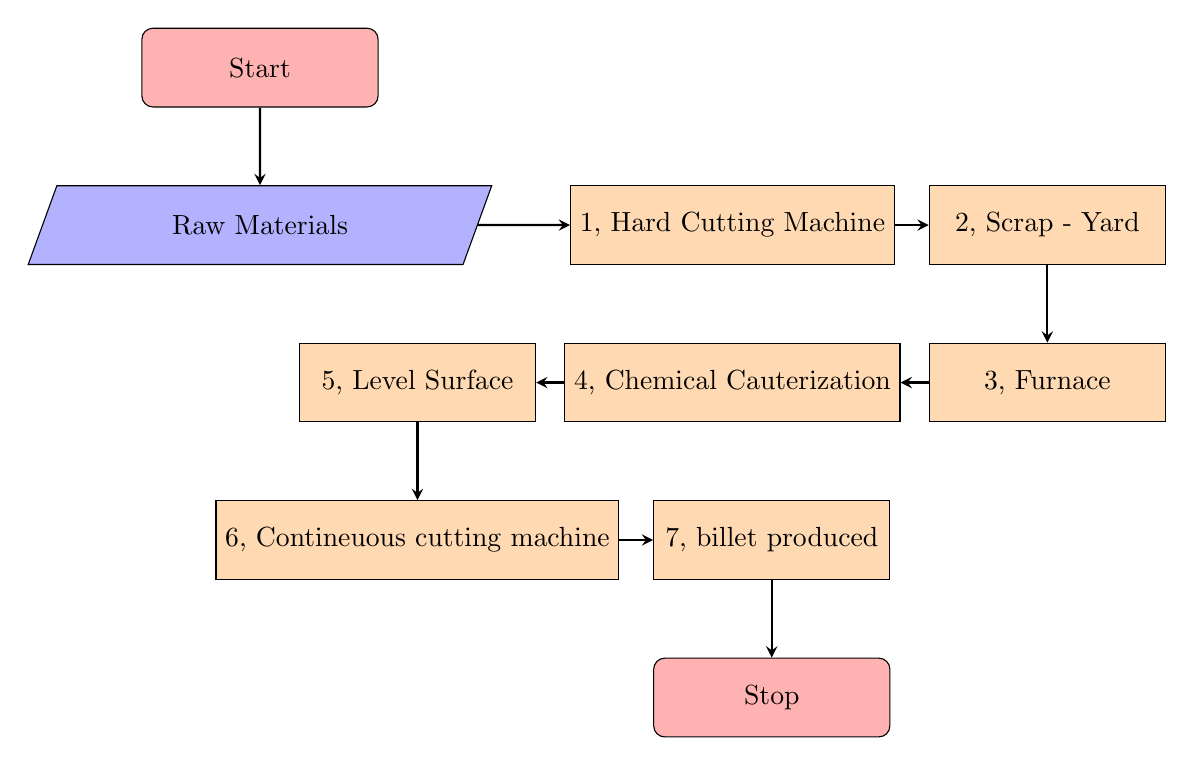
\begin{tikzpicture}[node distance = 2cm]
        	
        	\node[startstop,xshift = 2cm](start){Start};
        	\node[io,below of =start](input){Raw Materials};
        	\node[process,right of =input,xshift = 4cm](Process 1){1, Hard Cutting Machine};
        	\node[process,right of =Process 1,xshift = 2cm](Process 2){2, Scrap - Yard};
        	\node[process,below of =Process 2](Process 3){3, Furnace};
        	\node[process,left of =Process 3,xshift = -2 cm](Process 4){4, Chemical Cauterization};
        	\node[process,left of =Process 4,xshift = -2cm](Process 5){5, Level Surface};
        	\node[process,below of =Process 5](Process 6){6, Contineuous cutting machine};
        	\node[process,right of =Process 6,xshift = 2.5cm](Process 7){7, billet produced};
        	\node[startstop,below of =Process 7](stop){Stop};
        	
        	\draw [arrow](start)--(input);
			\draw [arrow](input)--(Process 1);
			\draw [arrow](Process 1)--(Process 2);
			\draw [arrow](Process 2)--(Process 3);
			\draw [arrow](Process 3)--(Process 4);
			\draw [arrow](Process 4)--(Process 5);
			\draw [arrow](Process 5)--(Process 6);
			\draw [arrow](Process 6)--(Process 7);
			\draw [arrow](Process 7)--(stop);
        	 
        	
        
        
        \end{tikzpicture}
        
             \begin{itemize}
        
\item(1){ 1 person control this step for proper cutting of raw materials}
\item(2){ after cutting 2 person takes the  materials from scrapyard to the furnace, the material is transferred to the furnace using a crane operated by one person } 
\item(3){ 2- 3 monitor and control the furnace }
\item(4){ 2 person apply chemical cauterization on the melted materials of the furnace}
\item(5){ 2 person level the melted materials coming from the furnace}
\item(6){ 2 person cuts the materials into equal chops of billet}
\item(7){ billet is produced}
\item{ transition between some of the process are done through crane which are operated by person}

        \end{itemize}
         \subsection{Drug international medicine}
        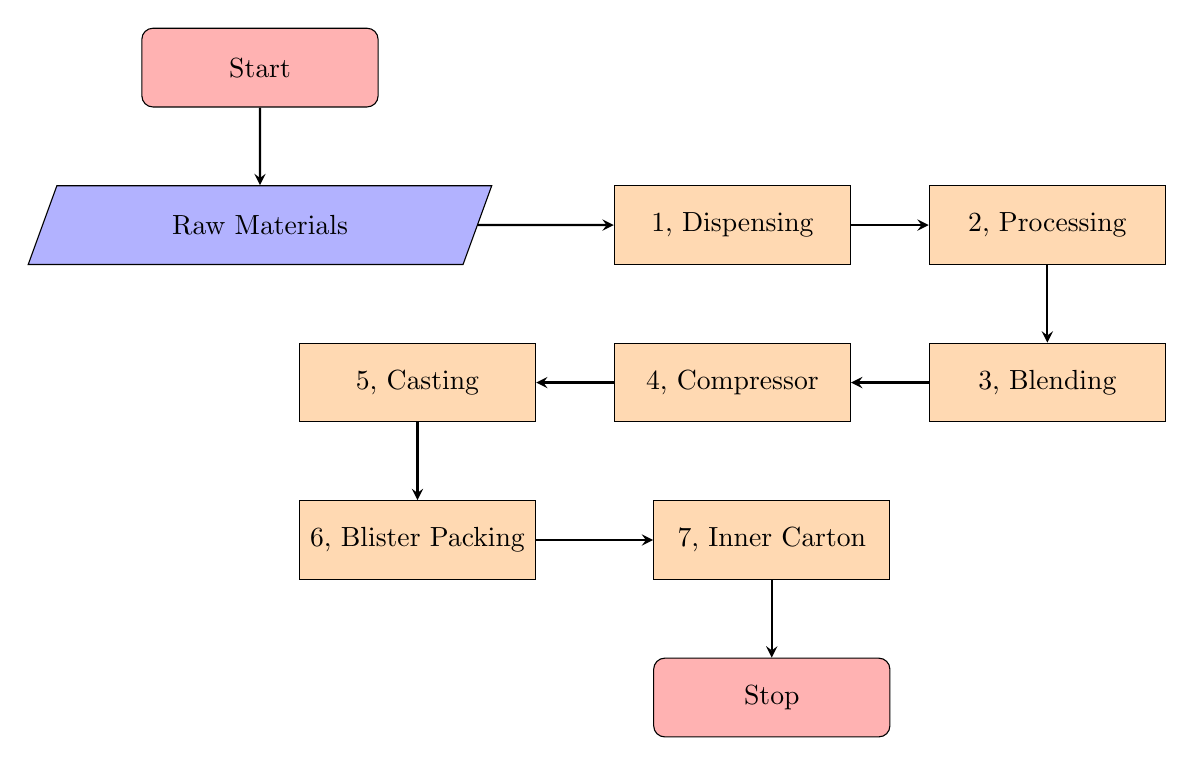
\begin{tikzpicture}[node distance = 2cm]
        	
        	\node[startstop,xshift = 2cm](start){Start};
        	\node[io,below of =start](input){Raw Materials};
        	\node[process,right of =input,xshift = 4cm](Process 1){1, Dispensing};
        	\node[process,right of =Process 1,xshift = 2cm](Process 2){2, Processing};
        	\node[process,below of =Process 2](Process 3){3, Blending};
        	\node[process,left of =Process 3,xshift = -2 cm](Process 4){4, Compressor};
        	\node[process,left of =Process 4,xshift = -2cm](Process 5){5, Casting};
        	\node[process,below of =Process 5](Process 6){6, Blister Packing};
        	\node[process,right of =Process 6,xshift = 2.5cm](Process 7){7, Inner Carton };
        	\node[startstop,below of =Process 7](stop){Stop};
        	
        	\draw [arrow](start)--(input);
			\draw [arrow](input)--(Process 1);
			\draw [arrow](Process 1)--(Process 2);
			\draw [arrow](Process 2)--(Process 3);
			\draw [arrow](Process 3)--(Process 4);
			\draw [arrow](Process 4)--(Process 5);
			\draw [arrow](Process 5)--(Process 6);
			\draw [arrow](Process 6)--(Process 7);
			\draw [arrow](Process 7)--(stop);
        	 
        	
        
        
        \end{tikzpicture}
        
             \begin{itemize}
        
\item(1){ 2 person control this step one weights the raw materials one takes the raw material to the next step }
\item(2){ 2 person maintains this step one drys the materials and the other puts in the blender
} 
\item(3){ 1 person controls the blending }
\item(4){ 1 person controls the compression}
\item(5){ 3 person is assigned to casting}
\item(6){ 1 person operates the machine 2 person checks the blister packing}
\item(7){ 3 person checks the carton packing}


        \end{itemize}
        
        
      
        	

 \section{Smart Manufacturing:}
       Smart manufacturing is a present trend in market that is continuously growing with time.Major forces driving smart manufacturing in manufacturing market are the growing need for centralized monitoring and predictive maintenance of manufacturing infrastructure. The increasing need for agile production, operational efficiency, and control, and demand-driven supply chain and connected logistics are also expected to drive the market.At present we are able to collect data using different types of sensor data due to wide spread of cloud technology. Cloud technology allow us to collect data in large volume and this data enable us to us to push toward smart manufacturing to answer questions like ''what to do" and "when to do it".The only threat existing in data driven technology is security.	Smart manufacturing can be divide into three parts
       
        	     \begin{itemize}
        
\item{Product and control solution: This include automation parts and products}
\item{IT solution enablers: power the whole concept of IoT and asset management. They help in building control, monitoring and analytics infrastructures.
} 
\item{Connectivity solution: servers,wan,router and wifi for smooth transition of data.}

				\end{itemize}
	
	
       \section{Data Driven Intelligence :}
       		Data driven intelligence is the forefront of industry at present.The advancement of machine learning techniques bloomed new possibilities of efficiency maximization never approached before.Machine learning allowed us to develop techniques to analyze data that are non-linear, which plagued the manufacturing industry for a long time but as time progressed it was evident that non linearity was not the only problem of developing smart manufacturing. Machine learning algorithm worked better on a hand picked features, but the massive data in smart manufacturing imposed a series of challenges to overcome like the present of multimodal data, high dimension of feature space and mutlicollinearity among measured data.This complications profoundly hinder the performance of the traditional machine learning algorithms.To properly address this challenges and issues, deep learning emerged as a new solution to handling and analyzing this big data.
       		
       		Deep learning allowed us to derive meaningful insights and features from complex and massive data. The idea behind deep learning is divide and conquer using mathematical mapping like a filter to co-ordinate a balance between linearity and non-linearity in data. Deep learning allowed us to develop high performance models using data where we do not use the handcrafted features.
       		
        	The use of such algorithms would allowed us to derive patterns from data and give meaningful insight and decisions.The key areas of manufacturing where it is useful
        	   
             \begin{itemize}
        
\item{ Product Company: Product life-cycle logistics and product design data tractability }
\item{ Manufacturer: Process control,shorter down time configuration flexibility and tractability.
} 
\item{ Supplier: Remote Diagnostics maintenance and improve availability }



        \end{itemize}
        
        \section{Data Collection:}
        	Data can be collected in many ways and the ability to collect this huge volume of data allows us to make decision that maximizes factory efficiency. A manufacturing factory works in  various small segmented areas to produce their product and for such reason it is possible for us to collect data from all this areas that co-depend to complete the whole manufacturing process.This areas include 
        	     \begin{itemize}
        
\item{Object or Product: Product number progress and products parts}
\item{Equipment: Sensor data and abnormalities in production. 
} 
\item{Process: Total performance of the whole process and it's quality}
\item{People: Gps location and its location activities}
\item{Environment: The temaperature,humdity and usage volume measurement}
				\end{itemize}
			Data collected in this manner are non-linear,multi-modal,Non-structured, has high volume and Mulit-formatted.Through various data cleaning techniques we structure it into our desirable form.Some of those techniques are removal of duplication,prediction of missing values,removal of corrupted data,scouting and removal of false data sets.
				
  		\section{Decisions and Analytics:}
  		So far we know the areas to collect data from and the areas to use those data on but one question remains, what are the things we would answer and how that will benefit the manufacturing process.In every manufacturing factory the key to maintaining a efficient flow of production is making the right decision at the right time, delay in taking initiative or making the right call can incur loss in large proportion.The answers to the questions that we need are mainly to make those calls are 
  		
  		\begin{itemize}
        
\item{Descriptive: Capture product condition,environment and operation}
\item{Diagnostic: Examine the causes of reduced product performance and detect failure. 
} 
\item{Predictive: Predict product quality and patterns that signal impending events}
\item{Prescriptive: Identify measure to improve outcome of correct problems}
	\end{itemize}
		Above points answers question like what happened,why it happened, what will happened and what are the action to take.This questions reveal a big picture about the manufacturing process and give us enough information to make informative decision at the nick of time.This answers were hard to predict in the sense that data collected for answering this question were complex in nature and could not be answered accurately with traditional machine learning algorithms.Deep learning paved the way for us to answer this questions using data which are high in velocity, variety and volume.
      \section{Possible Approaches of Data Analytics:}  
      So, to apply any data analytics  to increase efficiency first we need to collect data.The possible ways to properly collect the meaningful data is through various types of sensors.
      
      firstly to keep track of products produced we could use an radio-frequency identification for each product this allows us to detect the number of products manufactured with respect to time. This give us insight about the production rate so, in any case if production drops we would be able to easily identify when it happened.This tracking of product also allows us scale our production based on demand improving logistics support and supply management.
      
      Secondly, the machines follow a steady frequency while its in production, so with the help of an accelerometer we would be able to produce a time-series signal of the machine, thus giving a us monotonous pattern about the machine in work.In the case of any faults the vibration should change for example lose bearing,faults in motor etc.The time series data acquired through such means could be analyzed with Convolution neural network to extract temporal features while  Long short-term memory could be used to analyze the features as Lstm allows keeps previous information to make decision or we could use wavelet to derive features from this signal and then use Lstm to analyze the data further.
      
      Thirdly, data about people and their activities, it could be done through few means these are 
       	\begin{itemize}
        
\item{Camera: We could use image processing to determine their activities and how they control the machines using their computer in order to always look for possible errors or mistake made by the workers that could halt or hamper the production process. }
\item{eSense: It is a tool that allows us to monitor various human interactions and activities using a small wearable device.This device give use few information about the use like stress and emotion in voice, is he standing or walking, which direction he is looking and the position of the wearer inside the factory.
} 

	


	\end{itemize}
	Lastly,the room temperature and electricity data should be collected.Wrong room temperature might ruin the product quality and 
high electric consumption could increase the production cost significantly.
	We can analyze all this data to answer questions like what happened, why it happened, what will happen and what action to take.
	\section{Factory Operating in Different Dimension:}
	Lets consider a factory where production occurs in a daily basis, a factory of such manner can be divided into various dimension.These are mainly
	 	\begin{itemize}
        
\item{Finance: This portion of the section deals with the financial accounting, the data in this dimension are collected in form of balance sheets, income sheets and cash flow statements }
\item{People: This dimension deals with issues like office culture, work stress, customer feedback in product development and  work safety data collected in this sector is like number of workers and work schedules} 
\item{Process: the method of changing or combining the raw materials into the desired substance or product falls under process.This dimension deals with things such as quality control, job scheduling,repair and maintenance, machine operations and flexibility.This dimension give us the opportunity to collect in various form to transform the whole manufacturing process smart and efficient.}
\item{Product: This part of the dimension deals with logistics, packaging and time to market.
}
\item{Strategy: This is the most important dimension in the case of increasing the efficiency of production.Data collected from the above dimension can be analyzed and utilized  to make key strategic decision.Analysis of data allows us to get performance metrics  and cost efficient methods of manufacturing.
 
}
\end{itemize}
	Data can be collected from all this dimensions in various ways and the methods of storage various depending on connectivity of the factory and the technology used by them
	\begin{center}
	
	
	\begin{tabu} to 0.8\textwidth { | X[c,] | X[c] | X[c] |  X[c]| X[c]| X[c]|}
	 \hline
	 Dimension & Novice & Beginner & Learner & Intermediate & Expert \\	
	 \hline
	 Finance & store financial data using spreadsheet & store financial data using hard drive & store financial data using shared HDs & store financial data using cloud & store financial data using fog \\
	\hline
	 People & store people’s data using spreadsheet & store people’s data using hard drive & store people’s data using shared HDs & store financial people’s using cloud & store people’s data using fog \\
	 \hline
	 Process & store process data using spreadsheet & store process data using hard drive & store process data using shared HDs & store process data using cloud & store process data using fog \\
	 \hline
	 Product & store Product data using spreadsheet & store Product data using hard drive & store Product data using shared HDs & store Product data using cloud & store Product data using fog \\
	 \hline
	 Strategy & - & - & - & - &-\\
	 \hline
	\end{tabu}
	\end{center}
\section{Smart Manufacturing and logistics:}
	Logistics is used more broadly to refer to the process of coordinating and moving resources – people, materials, inventory, and equipment – from one location to storage at the desired destination. The term logistics originated in the military, referring to the movement of equipment and supplies to troops in the field.
	
	 Smart Logistic is a logistics system, which can enhance the flexibility, the adjustment to the market changes and
will make the company be closer to the customer needs. This will make possible to improve the level of customer
service, the optimization of the production and make lower the prices of storage and production. As the Smart
Logistics will change accordingly to the actual technology driven, it has a time dependency and thus it is essential to
define the state of the art of the technology.

	An efficient and robust logistics in 4.0 will use this three important methods or technologies
	 
  		\begin{itemize}
        
\item{Resource Planning: keep track of all the resources using RFID to be aware of raw materials live}
\item{Warehouse management systems : To use RFID to track and manage delivered product, what was not delivered and to send the such information down the supply chain. 
} 
\item{Transportation management systems: RFID and eSensor can track car location, the products being delivered on the truck and car use stress level to monitor the whole transport in logistics}

	\end{itemize}

	
\end{normalsize}
  
\end{document}